% \section{Fusion Discussion} \label{app_sec:fusion_discussion}

Intuitively it makes more sense to prefer early fusion, to maximize the model's access to extra information \citep{izacard2020leveraging, karpukhin2020dense}.
However, this can also be a disadvantage, as the signal from the artefact can get lost during the long computation. In the case of an artefact which is the gold output of a similar query from the training data, later fusion makes more sense. This also allows for a degree of explainability. By examining the forward pass of the last function we could determine what the contribution of the artefact was to the produced output.

The decision of how late the fusion should be depends heavily on the artefact type.
The application of every function in the chain of computation projects the input to some latent space.
The final function $f_n$ is special because it projects the output of previous functions to the space of possible outputs for the whole model.
In this space, there is the prediction $\hat{y}$ and also the true output $y$.
The task performance metric is defined in this space.
During inference, adding an artefact should ideally move the prediction in the output space closer to the correct output.
Assuming $c$ is the intermediate computation and there are two (overloaded) functions that produce a prediction: $\hat{y}_x = f_n(c)$ and $\hat{y}_\xi = f_n(c,\xi)$.
In circumstances in which adding the artefact helps, $L(\hat{y}_\xi, y) < L(\hat{y}_x, y)$, where $L$ is a loss function such as cross-entropy.
This is illustrated in the first row of \Cref{fig:computation_projection} for $n = 2$.

Assume that we can create an inverse of the last projection and see where the correct output lies in the intermediate representation.
There may be multiple such $c_t: f_n(c_t) = y$ or none, if too much information was lost by the first projection $f_1$.
Further, assume that there is always at least one such $c_t$.
We may then define an intermediate loss $L_i$ for each model computation by measuring the distance of the partial computations to the back-projection.
Similarly to late fusion, we consider two overloaded functions that produce the intermediate representation $c_x = f_1(q)$ and $c_\xi = f_1(q,\xi)$. 
Adding the artefact then ideally moves the intermediate representation closer to the back-projection and reduces the intermediate loss: $L^i(c_\xi, c_t) < L^i(c_x, c_t)$.\footnote{In case of multiple elements that map to $y$, we can define a loss that considers the minimum distance to any of them: ${L^i}' = \min L^i(c, c_t)$. If there is no such element in the projection space, then we may consider the elements that project close to the target $C_t = \arg \min L(f_2(c),y)$.}

This is illustrated in the second row of \Cref{fig:computation_projection}, which depicts a model with only two computational steps: $f_2 \circ f_1$. 
Early fusion (second row) adds the artefact to $f_1$, while late fusion adds it in the next step.
For simplicity in the figure, we consider the standard $L^2$ distance loss between the points.
In both cases, adding the artefact reduced the target loss. For early function, the intermediate loss was also reduced and the target loss was lower.
This does not always happen and complex computations may still at some point project the intermediate computation to the same point regardless of whether an artefact was added earlier or not.
It may also be the case that training with artefacts takes a longer time and the intermediate loss is higher but that the presence of the artefacts will make the model converge to a better optimum (lower generalization error).

\begin{figure*}[ht]
    \center
    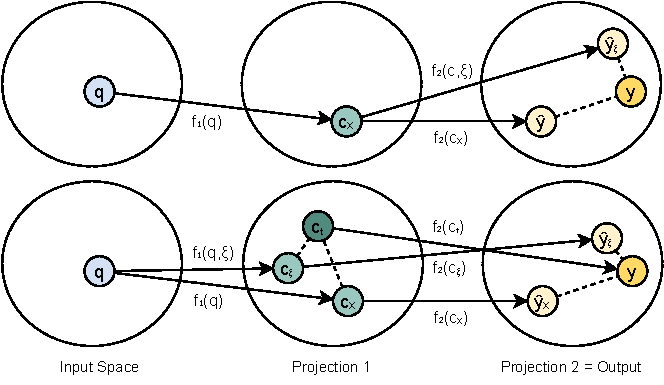
\includegraphics[width=0.95\textwidth]{img/computation_projection.pdf}
    \caption{Example of how late (top) and early (bottom) fusions affect the projections into intermediate spaces. The lengths of dashed lines correspond to the loss (longer is greater loss). Adding an artefact $\xi$ to the computation decreases the loss in both early and late fusions.}
    \label{fig:computation_projection}
\end{figure*}

Even though the invertibility of projections in this paper is only used as an illustration for the artefact fusion and an intermediate loss does not have to be defined in practice, invertible neural networks are an ongoing topic of research \cite{ardizzone2018analyzing, behrmann2020understanding}.
The combination of artefact retrieval and invertible neural networks has not yet been explored to our knowledge.